\tikzset{%
  >=latex
}
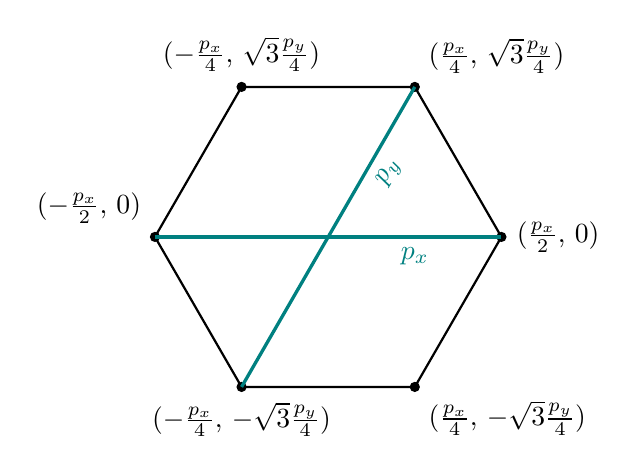
\begin{tikzpicture}[thick]
     \newdimen\R
     \R=2.2cm
     \draw (0:\R) \foreach \x in {60,120,...,360} {  -- (\x:\R) };
     \foreach \x/\l/\p in
       { 60/{($\frac{p_x}{4}$, $\sqrt{3} \frac{p_y}{4}$)}/above right,
        120/{($-\frac{p_x}{4}$, $\sqrt{3} \frac{p_y}{4}$)}/above,
        180/{($-\frac{p_x}{2}$, $0$)}/above left,
        240/{($-\frac{p_x}{4}$, $-\sqrt{3} \frac{p_y}{4}$)}/below,
        300/{($\frac{p_x}{4}$, $-\sqrt{3} \frac{p_y}{4}$)}/below right,
        360/{($\frac{p_x}{2}$, $0$)}/right
       }
       \node[inner sep=1pt,circle,draw,fill,label={\p:\l}] at (\x:\R) {};

       \draw[very thick, teal] (360:\R) -- (180:\R) node[near start, below] {$p_x$};

       \draw[very thick, teal] (240:\R) -- (60:\R) node[sloped, near end, below] {$p_y$};

\end{tikzpicture}
